
%% The first command in your LaTeX source must be the \documentclass command.
%%
%% Options:
%% twocolumn : Two column layout.
%% hf: enable header and footer.
\documentclass[
% twocolumn,
% hf,
]{ceurart}
\usepackage{amsmath,amssymb,longtable,hhline}
\usepackage{doi}
\def\doitext{DOI:}

%%
%% One can fix some overfulls
\sloppy

%%
%% Minted listings support
%% Need pygment <http://pygments.org/> <http://pypi.python.org/pypi/Pygments>
% \usepackage{listings}
\usepackage{minted}
\setminted{fontsize=\footnotesize,mathescape}
\usepackage{hyperref}

\hypersetup{
    bookmarks=true,         % show bookmarks bar?
    unicode=true,           % non-Latin characters in Acrobat’s bookmarks
    pdftoolbar=false,        % show Acrobat’s toolbar?
    pdfmenubar=false,        % show Acrobat’s menu?
    pdffitwindow=false,     % window fit to page when opened
    pdfstartview={FitH},    % fits the width of the page to the window
    pdftitle={},    % title
    pdfauthor={Evgeny Cherkashin},     % author
    pdfsubject={model driven architecture},   % subject of the document
    pdfnewwindow=true,      % links in new PDF window
    colorlinks=true,       % false: boxed links; true: colored links
    linkcolor=red,          % color of internal links (change box color with linkbordercolor)
    citecolor=green,        % color of links to bibliography
    filecolor=magenta,      % color of file links
    urlcolor=blue           % color of external links
  }

\usepackage{pifont}
\graphicspath{{pics/}}


%% auto break lines
% \lstset{breaklines=true}

\newcommand{\ns}[1]{\textbf{\texttt{#1}}}

%%
%% end of the preamble, start of the body of the document source.
\begin{document}

%%
%% Rights management information.
%% CC-BY is default license.
\copyrightyear{2021}
\copyrightclause{Copyright for this paper by its authors.
  Use permitted under Creative Commons License Attribution 4.0
  International (CC BY 4.0).}

%%
%% This command is for the conference information
\conference{2nd International Workshop on Advanced Information and Computation Technologies and Systems, December XX--XX, 2021, Irkutsk, Russia}

%%
%% The "title" command
\title{Technologies of Semantic WEB as an environment of application development and integration}
%%
%% The "author" command and its associated commands are used to define
%% the authors and their affiliations.
\author[1,2]{Evgeny A. Cherkashin}[%
orcid=0000-0003-2428-2471,
email=eugeneai@icc.ru,
url=https://github.org/eugeneai,
]
\address[1]{Matrosov Institute for System Dynamics and Control Theory of Siberian Branch of Russian Academy of Sciences, 134 Lermontov St, Irkutsk, 664033, Russian Federation}

\address[2]{Institute for Mathematics and Information Technologies, Irkutsk State University, 20~Gagarina Bulv, Irkutsk, 664003, Russian Federation}

%%
%% The abstract is a short summary of the work to be presented in the
%% article.
\begin{abstract}
  Semantic Web technologies and standards are becoming one of productive assets for software development and integration on various levels of design and implementation.  This include OSI level 6 data representation, database and file storage formats, the source data for indexes, hypertext markup, source data for document authoring, representing abstract software models, \emph{etc}.  They also smoothly combined with development and data analysis tools, giving raise a new common-ground environment for realizing integration on the semantic level.

  This paper presents the view on the Semantic Web technologies as data representation for software development tools with model analysis, transformation and retrospection capabilities.  Three examples are presented, exposing our experience.
\end{abstract}

%%
%% Keywords. The author(s) should pick words that accurately describe
%% the work being presented. Separate the keywords with commas.
\begin{keywords}
  knowledge graph \sep
  semantic web \sep
  model transformation \sep
  model-driven architecture \sep
  object-oriented logical programming \sep
  web application \sep
  geographical information system
\end{keywords}


%%
%% This command processes the author and affiliation and title
%% information and builds the first part of the formatted document.
\maketitle

\section{Introduction}

Since the beginning of 2000s the development of the Semantic Web technologies became [awesome] mostly in describing software domains, representing semantics withing data objects, and define first-order knowledge \cite{}.  A number of tools for automation of conceptual model design and model conversion were proposed as well \cite{}.  The R\&D at present is carried on in developing applications, improving and standardizing vocabularies, devising tools for solving particular problems.

Unification of routine tasks resulted in development common techniques for storing and processing data, which are aggregated around term ``knowledge graph'' (KG).  These include data representation formats, vocabulary standards, query languages, tools for accessing and management KG.  Software development techniques are mediated with properties of the new-created resources and their APIs\footnote{Abbreviation of Application Programming Interface}.  Many internet resources provide common ways of formalized domain data access using query endpoints, and these endpoints allow one to organize federated data access.

Domain specialists sometimes prefer develop local vocabularies instead of spending time for the routine work of Internet surfing for existing conceptual models and their enrichment.  This is due to underdevelopment of the metadata resources (meta vocabularies) due to lack a domain classification system as compared, \emph{e.g.} to Universal Decimal Classification (UDC) used in bibliography.  Vocabularies also can have common parts, describing the same or similar entities with different term or ways, more adopted to a specific problem solving.

Unitizing standardized vocabularies as domain conceptual models (ontologies) in our projects allow us to compare other research groups point of view to a problem with a formalized context, figure out underestimated and not fully formularized aspects of a domain under investigation/automation.  This is the similar information source as scientific papers, but having concrete formal presentation of the information objects, allowing one to get rid of particular uncertainties.  Another advantage of standardization is construction of a common ground of research, development, data formalization and interchange formats and semantics.  This include aggregation of results of pattern recognition, applications of machine learning with their following use as facts in knowledge-based systems.

The aim of this paper is to present a contemporary approach for SW and KG utilization in development applications in context of improving software developers and researchers performance.  A number of examples were reviewer showing advantageous points of the technologies application.


\section{Contemporary SW tools review}
\label{sec:sw-tools}

Semantic Web technologies from the developer point of view include the following assets:
\begin{enumerate}
\item Global identification of the entities via URI\footnote{Abbreviation of Universal Resource Identifiers}, IRI\footnote{Abbreviation of International Resource Identifier}, URL\footnote{Abbreviation of Universal Resource Locator}, which are essentially the same notions but reflecting different representation properties;
\item Conceptual set-theoretic and category-theoretic data representation as relation between resources and literals represented with triples of a form \texttt{<subject, predicate, object>};
\item Triples used in a description of a domain form a corresponding sematic graph, conditionally subdivided into terminological subgraph (T-Box) and instance subgraph (A-Box);
\item Graph presentation formats and techniques as files, databases, markups of documents, a data flow between applicants; \label{kg1}
\item Public vocabularies, mostly A-Boxes (databases), for example \texttt{DBPedia.org}, a formalized version of \texttt{Wikipedia.org}. % wikidata
\item For graphs being databases a query services are implemented to allow users obtain its data by portions, as well as implement modifications;
\item API and libraries for processing files and documents with semantic data acquisition (\emph{e.g.} by extraction of the markup).
\item Software for graph data processing;
\item Validation and verification services allowing one to explore correctness and consistency of the technologies use and domain conceptual models. \label{kg2}
\end{enumerate}
The assets \ref{kg1}--\ref{kg2} form knowledge graph technological aspect of the SW that gained in the last decade special R\&D directions.

Each entity being described in SW has its unique IRI, which is its virtual or real internet address locating it, \emph{e.g.} in a document most usually in a context of other resource.  Using IRIs in applications solves fundamental problem of cross-domain and cross-application object identification and forming a basis of common data processing environment.  Entities of various abstract levels can be designated an IRI, including vocabulary definitions (\emph{namespaces}), data types, data containers (files, databases).

Triples are combination of two or three IRIs.  Subject and predicate are always IRIs.  Objects are either IRI or a literal.  Literals are values of basic types (numbers, strings, dates, \emph{etc.}), usually accompanied with metadata (type designator and/or a language tag).  Types are defined in a vocabulary \texttt{<\url{http://www.w3.org/2001/XMLSchema}\#>}, having well-known namespace abbreviation \ns{xs}\footnote{Hereafter, all well-known namespace names will be given after its IRI in brackets with bold monospace font.}.  Language tag is used to define string values taking into account its affiliation to a cultural context.  It is recognized with KG tools and utilized at presentation layers of the software.

Namespaces are convenient instruments of resource definition.  For example \verb|integer| literal \verb|42^^<http://www.w3.org/2001/XMLSchema#integer>| can be reduced to \verb|42^^xs:integer|, where \verb|xs| is namespace prefix of term \verb|integer|.  Most of KG representation formats allow to define a default namespace, which terms are used without prefix.   Almost any conceptual model of a domain represented as KG comprises entities taken from multiple vocabularies, and namespaces allow to specify the origin of a term.  Three-component tuple (triple) being outside its KG context sometimes added the fourth component, its KG IRI (quadruple).

Much R\&D efforts since 2001 \cite{tbl} were spend to develop SW data representation formats and their coupling with document representation. The simplest way to provide a printed document with semantic representation is pointing user of software agent to an URL serving the data.  But this approach requires to implement two different procedures for document generation and its metadata.  That's why a RDFa\footnote{Abbreviation of Resource Description Framework attribute language} has been developed.  It allows developer of XHTML\footnote{HTML structures with strict XML restrictions obeyed} documents to add semantic layer inside the document.  The semantic markup is represented with special attributes and their values.  The hierarchical structure of XHTML is a matrix of hierarchical structure of document entities semantic relations.  The layer is extracted by XHTML/RDFa processing libraries.  There are other formats having the same expression capabilities as RDF but used for other purposes: \texttt{N-triples}, \texttt{Turtle}, \texttt{Notation~3}, \texttt{JSON-LD}.  The last one is an efficient way of coupling SW and various generic data storage, indexing and processing services.

Among published global vocabularies, \texttt{DBPedia} was of most valuable for our projects.  It is used for concrete object or notion of physical world reference, \emph{e.g.} ``passport'' in law documents authoring \cite{}, naming (labeling) referenced objects in user interface with corresponding words in natural language \cite{github-db}.  Another useful resource is \texttt{Wordnet} converted in RDF triples.  It describes semantics of english words and various mutual relations.

Access by program agents to the global resources are standardized as well.  Each serious vocabulary have API access point (endpoints) of form
\verb|http[s]://<address>/sparql|\footnote{For example, see DBpedia access point at the URL \url{https://dbpedia.org/sparql}} supporting direct \texttt{GET}-queries returning a user form, and \texttt{SPARQL} \texttt{POST} query with answering \texttt{JSON} encoded tabular result.  The form is used to interactively test \texttt{SPARQL} queries before their incorporation in software agents.  All \texttt{SPARQL} endpoints support federated queries, \emph{i.e.} run subqueries on another servers.   For a personal user KG storage, a number of servers were developed, \emph{e.g.}, \texttt{GraphDB}, \texttt{Jena Fuseki}, \texttt{ClioPatria}.  Each has its extension engines.  \texttt{ClioPatria} extends with Prolog modules and allows one to implement KG processing on server side.

KGs and their subgraphs are programmatically processed using libraries developed for all papular programming environments.  KG is represented with triple or quadruple set object.  The set is traversed, triples are filtered according to various criteria.  Filters are defined usually as patterns, where each of the components either a free variable/placeholder or a concrete value (IRI, literal), which must mach exactly.   Some libraries allow one execute \texttt{SPARQL} queries locally.  KG are evolved with adding new triples, as well as removing irrelevant ones.  The resulting modified KG is stored as files and published on a server.  An example of a federated SPARQL query is presented in Figure~\ref{fig:sparql-ex1}, which results in counting parts classes as the first level of a three widget.  Each class is named in Russian if \texttt{DBPedia} contains a corresponding label.  Otherwise label is figured out of IRI.  This query is running at a local server and initiates a subquery to \texttt{DBPedia.org} endpoint.

\begin{figure}[bth]
  \centering
\begin{minted}{sparql}
PREFIX dbr: <http://dbpedia.org/resource/>
PREFIX owl: <http://www.w3.org/2002/07/owl#>
PREFIX rdfs: <http://www.w3.org/2000/01/rdf-schema#>
select * where {
  ?class rdfs:subClassOf <http://dbpedia.org/resource/Electronic_component> .
  bind(replace(strafter(str(?class),str(dbr:)),'_',' ') as ?class_name) .
  OPTIONAL {
    SERVICE <http://dbpedia.org/sparql> {
      ?class rdfs:label ?title .
      FILTER (
        langMatches(lang(?title), 'ru')
      )
    }
  }
} limit 100
\end{minted}
  \caption{Example of a federated SPARQL query usage in a electronic component database}
  \label{fig:sparql-ex1}
\end{figure}

Formalized representation of a domain, which is provided by SW techniques, is the basis of automatic  inference construction, thus modeling, \emph{e.g.}, problem-solving, resulting decision synthesis, theorem proving, domain verification.  The inference is implemented in various ways, all of them belong either to semantic inference, usually implemented as solving a corresponding CSP\footnote{Abbreviation of Constraint Satisfaction Problem}, or syntax-driven procedures that mediate the previous structures and infer one of special properties (Automatic Theorem Proving).  Theoretic research is being carried on classification the properties of vocabularies by complexity of verification and development software implementing it for these classes.  These software are parts of RDF-processing libraries and stand-alone system extensions.

Our interest is located in inferring new objects using logic programming from domain models represented as KGs.  It allows developer to combine KG processing with other inferences in the same programming paradigm.  SWI-Prolog programming language environment and Logtalk extension is used for the purpose.  SWI system has library for representing and processing KG, and Logtalk is used to realize transformations providing the inference.  Object-oriented properties of Logtalk enable one to cope with generic disadvantaged of RDF\footnote{Requirements of triple tuple data representation.} with encapsulation, manipulate knowledge sets with extension, inheritance and composition, and represent inference in a generalized form of objects sending messages to each other.


% TODO: Integration out of our architecture.

\section{General architecture of applications based on KG}
\label{sec:architecture}

Some general words about architectures .... related to WEB.  Modeled with component architecture.

In order to present the general architecture of application development, we have to briefly speak about KG definitions and properties.

% \subsection{Knowledge graph properties as application basis}
% \label{sec:kg-as-basis}

KGs changed the view point to the knowledge base as being a part of whole totality of knowledge, implying the obeying the global standards and techniques of its acquisition and processing \cite{hogan}.  The following outlines their definitions \cite{hogan}.
 \begin{itemize}
  \item Notions \emph{data} and \emph{knowledge} are converged into ``something is \emph{known}'';
  \item KG contains, in general, data, relations, and metadata;
  \item The same KG is being filled in and processed by different independent modules, \emph{e.g.}, withing SPARQL queries with UPDATE statements;
  \item KG fundamental software development allow to \emph{postpone} the formal definition of a data schema;
  \item There is three points of view to graph schemata: \emph{semantic}, which is aimed at generalization, \emph{validating}, reflecting semantic verification, checking completeness w.r.t. sets of predefined general relations, and \emph{emergent}, observed or deduced from exploitation experience, as a set of new generalized structures and \emph{refactoring} of the KG.
  \end{itemize}

\begin{figure}[bth]
  \begin{center}
    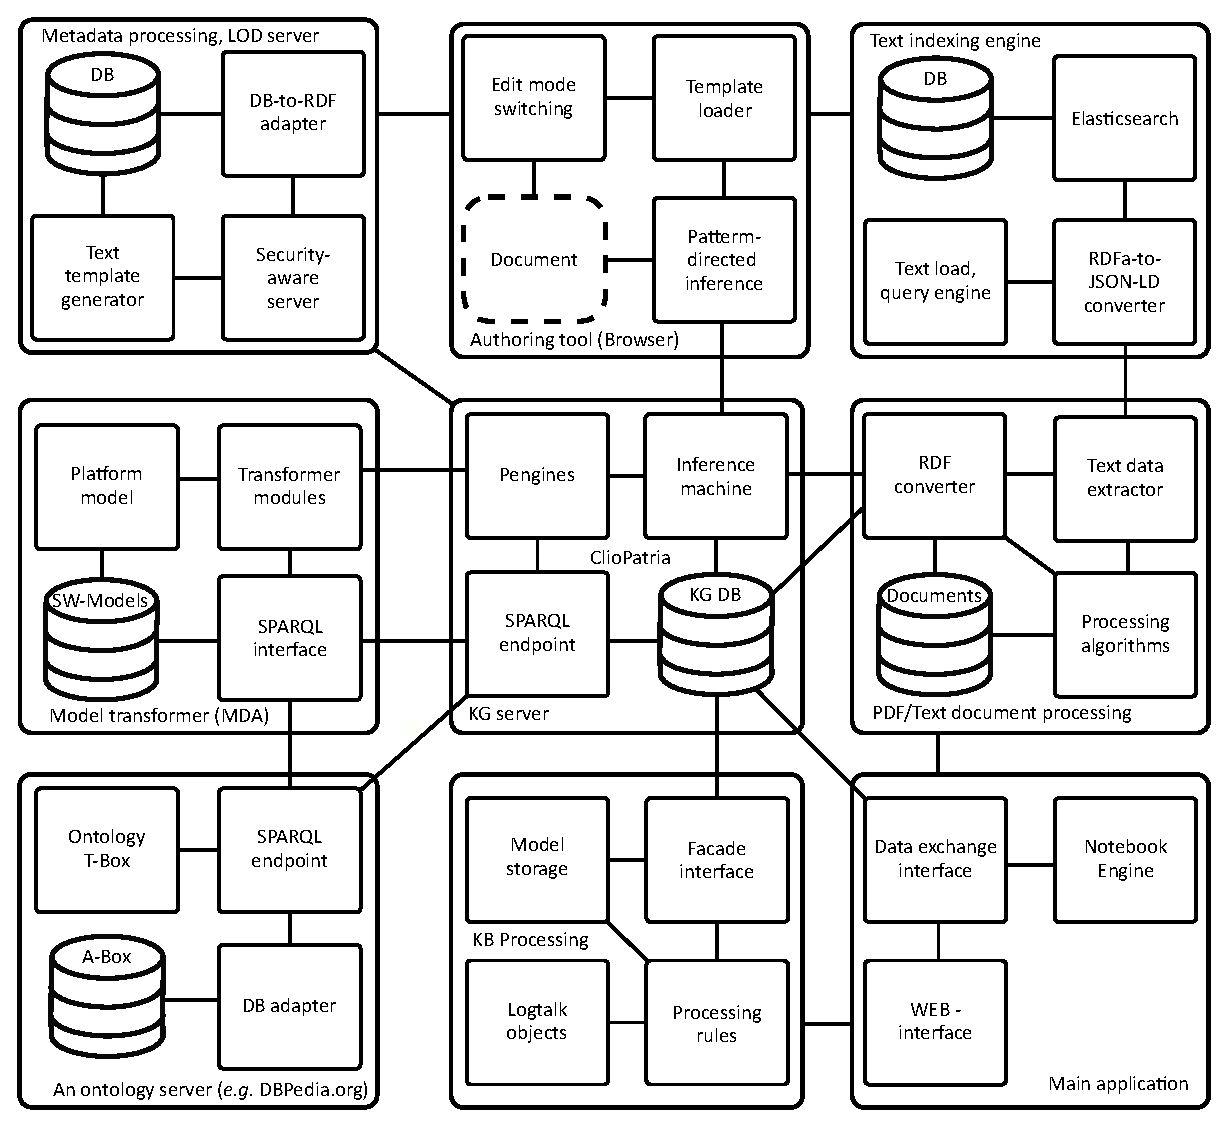
\includegraphics[width=0.9\linewidth]{architecture-mda-lod-ext-general.pdf}
  \end{center}
  \begin{center}
      \textbf{Abbreviations}\\[1ex]\scriptsize
      T-Module is Transformation module,
      MDA is Model-Driven Architecture,
      CIM is Computationally Independent Model,
      PIM is Platform Independent Model,
      PSM is Platform Specific Model,
      T-Box is Terminological Box,
      A-Box is Instance Box,
      A-Box is Instance Box,
      NGS is Next-Generation Sequencing,
      DB is Database.
  \end{center}

  \caption{Architecture of services}
  \label{fig:arch-services}
\end{figure}


\section{Discussion}
\label{sec:disc}


[we tried to collaborate with software developers using traditional approaches.  They are not interested as ]


CEUR-WS's article template provides a consistent \LaTeX{} style for
use across CEUR-WS publications, and incorporates accessibility and
metadata-extraction functionality. This document will explain the
major features of the document class.

If you are new to publishing with CEUR-WS, this document is a valuable
guide to the process of preparing your work for publication.

The ``\verb|ceurart|'' document class can be used to prepare articles
for any CEUR-WS publication, and for any stage of publication, from
review to final ``camera-ready'' copy with {\itshape very} few changes
to the source.

This class depends on the following packages
for its proper functioning:

\begin{itemize}
\item \verb|natbib.sty| for citation processing;
\item \verb|geometry.sty| for margin settings;
\item \verb|graphicx.sty| for graphics inclusion;
\item \verb|hyperref.sty| optional package if hyperlinking is required in
  the document;
\item \verb|fontawesome5.sty| optional package for bells and whistles.
\end{itemize}

All the above packages are part of any
standard \LaTeX{} installation.
Therefore, the users need not be
bothered about downloading any extra packages.

\section{Modifications}

Modifying the template --- including but not limited to: adjusting
margins, typeface sizes, line spacing, paragraph and list definitions,
and the use of the \verb|\vspace| command to manually adjust the
vertical spacing between elements of your work --- is not allowed.

\section{Template parameters}

There are a number of template
parameters which modify some part of the \verb|ceurart| document class.
This parameters are enclosed in square
brackets and are a part of the \verb|\documentclass| command:
% \begin{lstlisting}
%   \documentclass[parameter]{ceurart}
% \end{lstlisting}

Frequently-used parameters, or combinations of parameters, include:
\begin{itemize}
\item {\verb|twocolumn|}: Two column layout.
\item {\verb|hf|}: Enable header and footer\footnote{You can enable
    the display of page numbers in the final version of the entire
    collection. In this case, you should adhere to the end-to-end
    pagination of individual papers.}.
\end{itemize}

\section{Front matter}

\subsection{Title Information}

The titles of papers should be either all use the emphasizing
capitalized style or they should all use the regular English (or
native language) style. It does not make a good impression if you or
your authors mix the styles.

Use the \verb|\title| command to define the title of your work. Do not
insert line breaks in your title.

\subsection{Title variants}

% \verb|\title| command have the below options:
% \begin{itemize}
% \item \verb|title|: Document title. This is default option.
% \begin{lstlisting}
% \title[mode=title]{This is a title}
% \end{lstlisting}
% You can just omit it, like as follows:
% \begin{lstlisting}
% \title{This is a title}
% \end{lstlisting}

% \item \verb|alt|: Alternate title.
% \begin{lstlisting}
% \title[mode=alt]{This is a alternate title}
% \end{lstlisting}

% \item \verb|sub|: Sub title.
% \begin{lstlisting}
% \title[mode=sub]{This is a sub title}
% \end{lstlisting}
% You can just use \verb|\subtitle| command, as follows:
% \begin{lstlisting}
% \subtitle{This is a sub title}
% \end{lstlisting}

% \item \verb|trans|: Translated title.
% \begin{lstlisting}
% \title[mode=trans]{This is a translated title}
% \end{lstlisting}

% \item \verb|transsub|: Translated sub title.
% \begin{lstlisting}
% \title[mode=transsub]{This is a translated sub title}
% \end{lstlisting}
% \end{itemize}

\subsection{Authors and Affiliations}

Each author must be defined separately for accurate metadata
identification. Multiple authors may share one affiliation. Authors'
names should not be abbreviated; use full first names wherever
possible. Include authors' e-mail addresses whenever possible.

\verb|\author| command have the below options:

\begin{itemize}
\item \verb|style|: Style of author name (chinese)
\item \verb|prefix|: Prefix
\item \verb|suffix|: Suffix
\item \verb|degree|: Degree
\item \verb|role|: Role
\item \verb|orcid|: ORCID
\item \verb|email|: E-mail
\item \verb|url|: URL
\end{itemize}

Author names can have some kinds of marks and notes:
\begin{itemize}
\item affiliation mark: \verb|\author[<num>]|.
% \item email: \verb|\ead{<email>}|,
% \item url: \verb|\ead[url]{<url>}|.
\end{itemize}

The author names and affiliations could be formatted in two ways:
\begin{enumerate}
\item Group the authors per affiliation.
\item Use an explicit mark to indicate the affiliations.
\end{enumerate}

Author block example:
% \begin{lstlisting}
% \author[1,2]{Author Name}[%
%     prefix=Prof.,
%     degree=D.Sc.,
%     role=Researcher,
%     orcid=0000-0000-000-0000,
%     email=name@example.com,
%     url=https://name.example.com
% ]

% \address[1]{Affiliation #1}
% \address[2]{Affiliation #2}
% \end{lstlisting}

% \subsection{Abstract and Keywords}

% Abstract shall be entered in an environment that starts
% with \verb|\begin{abstract}| and ends with
% \verb|\end{abstract}|.

% \begin{lstlisting}
% \begin{abstract}
%   This is an abstract.
% \end{abstract}
% \end{lstlisting}

% The key words are enclosed in a \verb|keywords|
% environment. Use \verb|\sep| to separate keywords.

% \begin{lstlisting}
% \begin{keywords}
%   First keyword \sep
%   Second keyword \sep
%   Third keyword \sep
%   Fourth keyword
% \end{keywords}
% \end{lstlisting}

At the end of front matter add \verb|\maketitle| command.

\section{Sectioning Commands}

Your work should use standard \LaTeX{} sectioning commands:
\verb|\section|, \verb|\subsection|,
\verb|\subsubsection|, and
\verb|\paragraph|. They should be numbered; do not remove
the numbering from the commands.

Simulating a sectioning command by setting the first word or words of
a paragraph in boldface or italicized text is not allowed.

\section{Tables}

The ``\verb|ceurart|'' document class includes the ``\verb|booktabs|''
package --- \url{https://ctan.org/pkg/booktabs} --- for preparing
high-quality tables.

Table captions are placed \textit{above} the table.

Because tables cannot be split across pages, the best placement for
them is typically the top of the page nearest their initial cite.  To
ensure this proper ``floating'' placement of tables, use the
environment \verb|table| to enclose the table's contents and the
table caption. The contents of the table itself must go in the
\verb|tabular| environment, to be aligned properly in rows and
columns, with the desired horizontal and vertical rules.

Immediately following this sentence is the point at which
Table~\ref{tab:freq} is included in the input file; compare the
placement of the table here with the table in the printed output of
this document.

\begin{table*}
  \caption{Frequency of Special Characters}
  \label{tab:freq}
  \begin{tabular}{ccl}
    \toprule
    Non-English or Math&Frequency&Comments\\
    \midrule
    \O & 1 in 1,000& For Swedish names\\
    $\pi$ & 1 in 5& Common in math\\
    \$ & 4 in 5 & Used in business\\
    $\Psi^2_1$ & 1 in 40,000& Unexplained usage\\
  \bottomrule
\end{tabular}
\end{table*}

To set a wider table, which takes up the whole width of the page's
live area, use the environment \verb|table*| to enclose the table's
contents and the table caption.  As with a single-column table, this
wide table will ``float'' to a location deemed more
desirable. Immediately following this sentence is the point at which
Table~\ref{tab:commands} is included in the input file; again, it is
instructive to compare the placement of the table here with the table
in the printed output of this document.

\begin{table}
  \caption{Some Typical Commands}
  \label{tab:commands}
  \begin{tabular}{ccl}
    \toprule
    Command &A Number & Comments\\
    \midrule
    \texttt{{\char'134}author} & 100& Author \\
    \texttt{{\char'134}table}& 300 & For tables\\
    \texttt{{\char'134}table*}& 400& For wider tables\\
    \bottomrule
  \end{tabular}
\end{table}

\section{Math Equations}

You may want to display math equations in three distinct styles:
inline, numbered or non-numbered display.  Each of the three are
discussed in the next sections.

\subsection{Inline (In-text) Equations}

A formula that appears in the running text is called an inline or
in-text formula.  It is produced by the \verb|math| environment,
which can be invoked with the usual
\verb|\begin| \ldots \verb|\end| construction or with
the short form \verb|$| \ldots \verb|$|. You can use any of the symbols
and structures, from $\alpha$ to $\omega$, available in
\LaTeX~\cite{Lamport:LaTeX};
this section will simply show a few
examples of in-text equations in context. Notice how this equation:
\begin{math}
  \lim_{n\rightarrow \infty} \frac{1}{n} = 0,
\end{math}
set here in in-line math style, looks slightly different when
set in display style.  (See next section).

\subsection{Display Equations}

A numbered display equation---one set off by vertical space from the
text and centered horizontally---is produced by the \verb|equation|
environment. An unnumbered display equation is produced by the
\verb|displaymath| environment.

Again, in either environment, you can use any of the symbols and
structures available in \LaTeX{}; this section will just give a couple
of examples of display equations in context.  First, consider the
equation, shown as an inline equation above:
\begin{equation}
  \lim_{n\rightarrow \infty} \frac{1}{n} = 0.
\end{equation}
Notice how it is formatted somewhat differently in
the \verb|displaymath|
environment.  Now, we'll enter an unnumbered equation:
\begin{displaymath}
  S_{n} = \sum_{i=1}^{n} x_{i} ,
\end{displaymath}
and follow it with another numbered equation:
\begin{equation}
  \lim_{x \to 0} (1 + x)^{1/x} = e
\end{equation}
just to demonstrate \LaTeX's able handling of numbering.

\section{Figures}

The ``\verb|figure|'' environment should be used for figures. One or
more images can be placed within a figure. If your figure contains
third-party material, you must clearly identify it as such, as shown
in the example below.
\begin{figure}
  \centering
  % \includegraphics[width=\linewidth]{sample-franklin}
  \caption{1907 Franklin Model D roadster. Photograph by Harris \&
    Ewing, Inc. [Public domain], via Wikimedia
    Commons. (\url{https://goo.gl/VLCRBB}).}
\end{figure}

Your figures should contain a caption which describes the figure to
the reader. Figure captions go below the figure. Your figures should
also include a description suitable for screen readers, to
assist the visually-challenged to better understand your work.

Figure captions are placed below the figure.

\section{Citations and Bibliographies}

The use of Bib\TeX{} for the preparation and formatting of one's
references is strongly recommended. Authors' names should be complete
--- use full first names (``Donald E. Knuth'') not initials
(``D. E. Knuth'') --- and the salient identifying features of a
reference should be included: title, year, volume, number, pages,
article DOI, etc.

The bibliography is included in your source document with these two
commands, placed just before the \verb|\end{document}|
command:
% \begin{lstlisting}
% \bibliography{bibfile}
% \end{lstlisting}
where ``\verb|bibfile|'' is the name, without the ``\verb|.bib|''
suffix, of the Bib\TeX{} file.

\begin{acknowledgments}

  The results were obtained within the state assignment of the Ministry of Education and Science of Russia, the project ``Methods and technologies of a cloud-based service-oriented digital platform for collecting, storing and processing large volumes of multi-format interdisciplinary data and knowledge based on the use of artificial intelligence, a model-driven approach and machine learning'', No.~FWEW-2021-0005 (State registration No.~121030500071-2).

  The results obtained with the use of the network infrastructure of Telecommunication center of collective use ``Integrated information-computational network of Irkutsk scientific-educational complex'' (\url{http://net.icc.ru}).

The~R\&D on GIS-viewer of faults involved the Centre of Geodynamics and Geochronology equipment at the Institute of the Earth's Crust, Siberian Branch of the Russian Academy of Sciences (grant No.~075-15-2021-682).   This study direction was partially carried out within the basic budgetary research project ``Modern geodynamics, mechanisms of destruction of the lithosphere and hazardous geological processes in Central Asia'', No.~FWEF-2021-0009.

The~development of the~infrastructure for Mothur command transformation to Rapidminer dataflow diagram is supported by the project of Irkutsk scientific center of Siberian branch of Russian Academy of sciences, grant No 4.2.

\end{acknowledgments}
%%
%% Define the bibliography file to be used
% \bibliography{sample-ceur}

\begin{thebibliography}{99}

\bibitem{tbl} T.B.-L. Scientific American ...

\bibitem{lod} C.~Bizer, T.~Heath, T.~Berners-Lee, Linked Data -- The Story So Far. Int. J. Semantic Web Inf. Syst., 5 (2009), pp.~1--22. \doi{10.4018/jswis.2009081901}

\bibitem{lunina} O.~V.~Lunina.  The digital map of the Pliocene–Quaternary crustal faults in the Southern East Siberia and the adjacent Northern Mongolia. Geodynamics \& Tectonophysics.  V.~7(3) (2016). pp.~407-434. (in Russian) \doi{10.5800/GT-2016-7-3-0215}

\bibitem{hogan} A.~Hogan, E.~Blomqvist, M.~Cochez, C.~D’Amato \emph{et al}. Knowledge Graphs, 2020. \url{https://arxiv.org/abs/2003.02320v5}

\bibitem{afs} A.~A.~Gladkov, O.~V.~Lunina. Cartographic service ``Activetectonics''. \url{http://activetectonics.ru/} (access date: 20-Sep-2021)

\bibitem{foss} M.~Leidig, R.~Teeuw. Free software: A review, in the context of disaster management. International Journal of Applied Earth Observation and Geoinformation, 42 (2015), pp.~49-56. \doi{10.1016/j.jag.2015.05.012}.

\bibitem{lgd} C.~Stadler, J.~Lehmann, K.~Höffner, S.~Auer. LinkedGeoData: A core for a web of spatial open data. Semantic Web 3 (2012) 333–354. \doi{10.3233/SW-2011-0052}

\bibitem{geolink} M.~Cheatham, A.~Krisnadhi, R.~Amini, P.~Hitzler, \emph{et al}. The GeoLink knowledge graph, Big Earth Data, 2:2 (2018), pp.~131-143. \doi{10.1080/20964471.2018.1469291}

\bibitem{abid} T.~Abid, H.~Zarzour. Integrating linked open data in geographical information system. Procs. of. International Conference on Information Technology for Organization Development. Oct 19-20, 2014, University of Tebessa, Tebessa, Algeria (2014).

\bibitem{iwaniak1} A.~Iwaniak, I.~Kaczmarek, M.~Strzelecki, J.~Lukowicz, P.~Jankowski. Enriching and improving the quality of linked data with GIS. Open Geosciences, Vol.~8, 1~(2016) pp.~323-336. \doi{10.1515/geo-2016-0020}

\bibitem{iwaniak17} A.~Iwaniak, M.~Leszczuk, M.~Strzelecki, F.~Harvey, I.~Kaczmarek. A Novel Approach for Publishing Linked Open Geodata from National Registries with the Use of Semantically Annotated Context Dependent Web Pages. International Journal of Geo-Information. 6, 252 (2017). \doi{10.3390/ijgi6080252}

\bibitem{zont19} E.~Cherkashin, A.~Shigarov, V.~Paramonov. Representation of MDA transformation with logical objects. International Multi-Conference on Engineering, Computer and Information Sciences (SIBIRCON), Novosibirsk, Russia. (2019) 0913--0918 \doi{10.1109/SIBIRCON48586.2019.8958008}

\bibitem{authoring} E.~Cherkashin, A.~Shigarov, V.~Paramonov, A.~Mikhailov, Digital archives supporting document content inference, Procs. of 42-nd International Convention on Information and Communication Technology Electronics and Microelectronics (MIPRO), May, 20–24, 2019. pp. 1037-1042. \doi{10.23919/MIPRO.2019.8757196}

\bibitem{gisviewer} E.~Cherkashin, O.~Lunina, L.~Demyanov, A.~Tsygankov. Web-GIS viewer for active faults data represented as a knowledge graph. Proceedings for 4th Scientific-practical Workshop Information Technologies: Algorithms, Models, Systems. Irkutsk, Russia, September 14, 2021. CEUR-WS.org, online \url{http://ceur-ws.org/Vol-2984/paper8.pdf}

\end{thebibliography}
\section{Online Resources}

The sources for the viewer are being developed at Github, URL:~\url{https://github.com/De17eon/GRL}.

\end{document}

%%
%% End of file


%%% Local Variables:
%%% mode: latex
%%% TeX-master: "paper-aicts-cherkashin.tex"
%%% End:
